\section{Implementation challenges} \label{chap:challenges}

During the whole implementation process we've faced a significant amount of challenges of a diverse nature. For a major part of them we were able to find a feasible solution that was implemented or at least managed to come up with some solution propositions. All the challenges can be split up in the application categories, which are listed below.

\subsection{Organizational challenges}

\begin{enumerate}
  \item Organization of groups
  \begin{itemize}
      \item Problem encountered:\\
      The main problem from the beginning of the practical course was to organize all the project members into equally skilled groups. The splitting principles were also not clear.
      \item Solution found:\\
      The first solution we came up with was to split up into two groups of three people, which proved efficient enough (or rather the inconveniences didn't show up) at the initial working stages such as acquiring the initial knowledge and getting familiar with the tools. After some time it became clear, that this group separation doesn't work anymore. Because the workload of the whole project which stretched throughout the remaining time was too much for three people to carry out, so it was decided to unite the groups and continue working on the project jointly. This changing of structure mid-project also led to further complications in regards to management within a group, which will be discussed next.
  \end{itemize}
  \item Organization and management within a group
   \begin{itemize}
      \item Problem encountered:\\
        In terms of the management within the group, the major problems that were encountered are: \\
        - Lack of high-level working plan and working structure that everyone can stick to.\\
        - No clear role assignment for the project members, lack of the task management.\\
        - Lack of day-to-day updates and communication.\\
        - No unified repository for everyone to work with and further complications tied with that (follows the problem with groups separation mentioned previously)
      \item Solution found:\\
        The solution that helped to fix (to some degree) the first two problems was to (following the unification of two groups into one single unit) get rid of the multitasking paradigm  and to assign some specific task or "area of expertise" to each member of the project. Thus, after such decentralization the need for a centralized high-level working plan was decreased, because each participant could organize the working process to fulfill own needs the best. This of course led to deepening the problem of lacking communication and the solution was not the most efficient in terms of implementation speed. 
        The communication problem - tied to the absence of a single unified repository for each project member to work with - was solved in the second half of the project using GitHub.

  \end{itemize}
\end{enumerate}

\subsection{Software design challenges}
\begin{itemize}
    \item PID loop tuning: 
     \begin{itemize}
      \item Problem encountered:\\
    We could not perform any tests to find the optimal PID gains since the robot was not assembled and the new microcontroller cannot be implemented on a breadboard. The same issue also applied to the other peripherals.
      \item Solution found:\\
    we performed the PID loop tuning by adapting the code to run on the the disPIC30F microcontroller mounted on a breadboard with one wheel. This solution is not optimal, since the final weight of the robot could change the parameters but it gives a reasonable estimate for our problem. For some peripherals, like the timer, we could run simulations to validate them, but for others like the ADC converter we are still uncertain how it would perform once the board is actually assembled.
        \end{itemize}
\end{itemize}

\subsection{PCB design challenges}
\begin{enumerate}
  \item Missing knowledge of a PCB
    \begin{itemize}
      \item Problem encountered:\\
      As it was mentioned in earlier stages of this document, at the beginning of this project, all of us didn't know how to design or even build a PCB board due to lack of knowledge in electrical engineering. 
      \item Solution found:\\
      During the practical course we learned the basics of how a schematic has to look like by rebuilding the schematic of the "dsPIC30F4011 Prototype Design" from scratch onto a breadboard. We sometimes also had to have a look at lasts year's micromouse PCB board for reference of placing several parts. 
    \end{itemize}
  \item Design of the final schematic and PCB
    \begin{itemize}
      \item Problem encountered:\\
      The overall process of designing the complete board took at approx. five to six weeks, which is far too long than we had anticipated. One of the main issues was the identification of the correct electronic components we needed for the board. The constraint was to only order parts from RSComponents, but not every component we had found was offered by them.
      Another time-consuming act was the decision of how to place all components so their elecromagnetic interference won't interfere with each other.
      \item Solution found:\\
      Most of the components we needed were already used by us in the practical course, hence we could copy them and their placement from the "dsPIC30F4011 Prototype Design" schematic. The main difference was that we changed the microcontroller to a dsPIC33FJ64MC804 - with almost double the amounts of pins, which didn't made it easier to design. But still we had to find a proper way of placing all components on the PCB which doesn't take too much space and doesn't lead to interfering parts.
    \end{itemize}
  \item Tracing of the PCB
    \begin{itemize}
      \item Problem encountered:\\
      We had to take into account the limited space we had on the board plus the correct size of the tracing for the several circuits. For example the tracing for the 9V battery circuit had to be bigger in size because of the higher possible current than on the 5V and 3.3V circuits.
      Another difficulty was to connect all pins according to the schematic due to the high amount of traces we needed. The finishing touch was to draw traces by using as few as possible vias.
      \item Solution found:\\
      After revising each iteration after another and talking to our professor, we finally reached a final state which was satisfactory for all of us. Although not all vias could be avoided, in the end we created a clean layout for the tracing.
    \end{itemize}
  \item Using Autodesk Eagle
    \begin{itemize}
      \item Problem encountered:\\
      Autodesk Eagle is a huge software environment for creating schematics and its counterpart the PCB - which no one of the team had ever used before. This means that we encountered a lot of problems on how to find the correct parts within the "Parts Library" and later on in the added "SamacSys Library". We had difficulties in selecting the correct parts which we used later on in the final version, and no idea whether the placement of the components is right or not. 
      \item Solution found:\\
      Through self-learning and literally trying out functionalities we managed to use Eagle as we pleased. In the end we had two experts for Eagle within our team, which did the part selection, placement and tracing of the components.
    \end{itemize}
\end{enumerate}

\subsection{Casing design challenges}

\begin{enumerate}
  \item Coordination with PCB Design
  \begin{itemize}
      \item Problem encountered:\\
      For design processes that are in parallel to each other, it is unavoidable to go back and forth. The challenge is to make modifications to the design without causing too much unnecessary work, as these modifications can happen quite frequently and making changes to existing design can often be error-prone.
      \item Solution found:\\
      One solution is to take advantage of “Parameters” feature of Fusion 360. To effectively utilising this feature, we need to make sure that non-critical dimensions are built upon these selected ones in a logical fashion, this is the key idea of parameter centric design approach. Since Fusion 360 provides an easy interface for modifying set parameters and automatically updates any design dimensions that are constrained upon these parameters, it can be a chain reaction after each modification to parameters. A set of effectively selected parameters not only ensures that we can modify the design according to our needs even later in the process, but also eliminates or at least minimises excessive manual modification.
      
      For example, when choosing the position of the motor’s central point, there are many things that can influence or change our decision, such as the dimension of the wheel and the clearance height from the floor that is necessary. One logical thing to do is to design the motor mount, through holes for the screws fastening the motor based on this motor position and set this position as our “parameter”. In this way if the wheel’s dimension is somehow changed, and we need to change the position of the motor, only slight modification to this “parameter” is needed, and Fusion 360 will automatically update the position of the motor mount etc.
  \end{itemize}
  \item Design for Tolerance
  \begin{itemize}
      \item Problem encountered:\\
      Any mechanical design of parts needs to take into account tolerance of dimensional errors. With the FDM 3D printer that we used providing a dimensional accuracy of lower limit of around $\pm$ 0.5 mm, and ordered parts such as the distance sensor having a (default) tolerance of $\pm$ 0.3 mm \cite{sens}, it is worth paying attention when designing for fitting these parts to the casing.
      \item Solution found:\\
      The solution is quite straightforward, it is to design for the maximum error, and leave enough room for a tight fit. One exception is the case snap fit, where the clearance between two fit structures is 0.5 mm as recommended in \cite{low}.
      
  \end{itemize}
  \item Design for 3D Printing
  \begin{itemize}
      \item Problem encountered:\\
      3D printing is a relatively fast and cheap way to produce prototypes, but it comes with its limitations. The 3D printing method we used (FDM) requires certain support structures to be added if there are steep overhanging parts, because heated and fluid material can not be deposited onto thin air. Without support structure, the print would deform and sometimes cause print fail. If support structures are used, removing such structures will leave the surface rough.

\begin{figure}[htb]
    \centering
    \begin{minipage}{.45\textwidth}
          \centering
            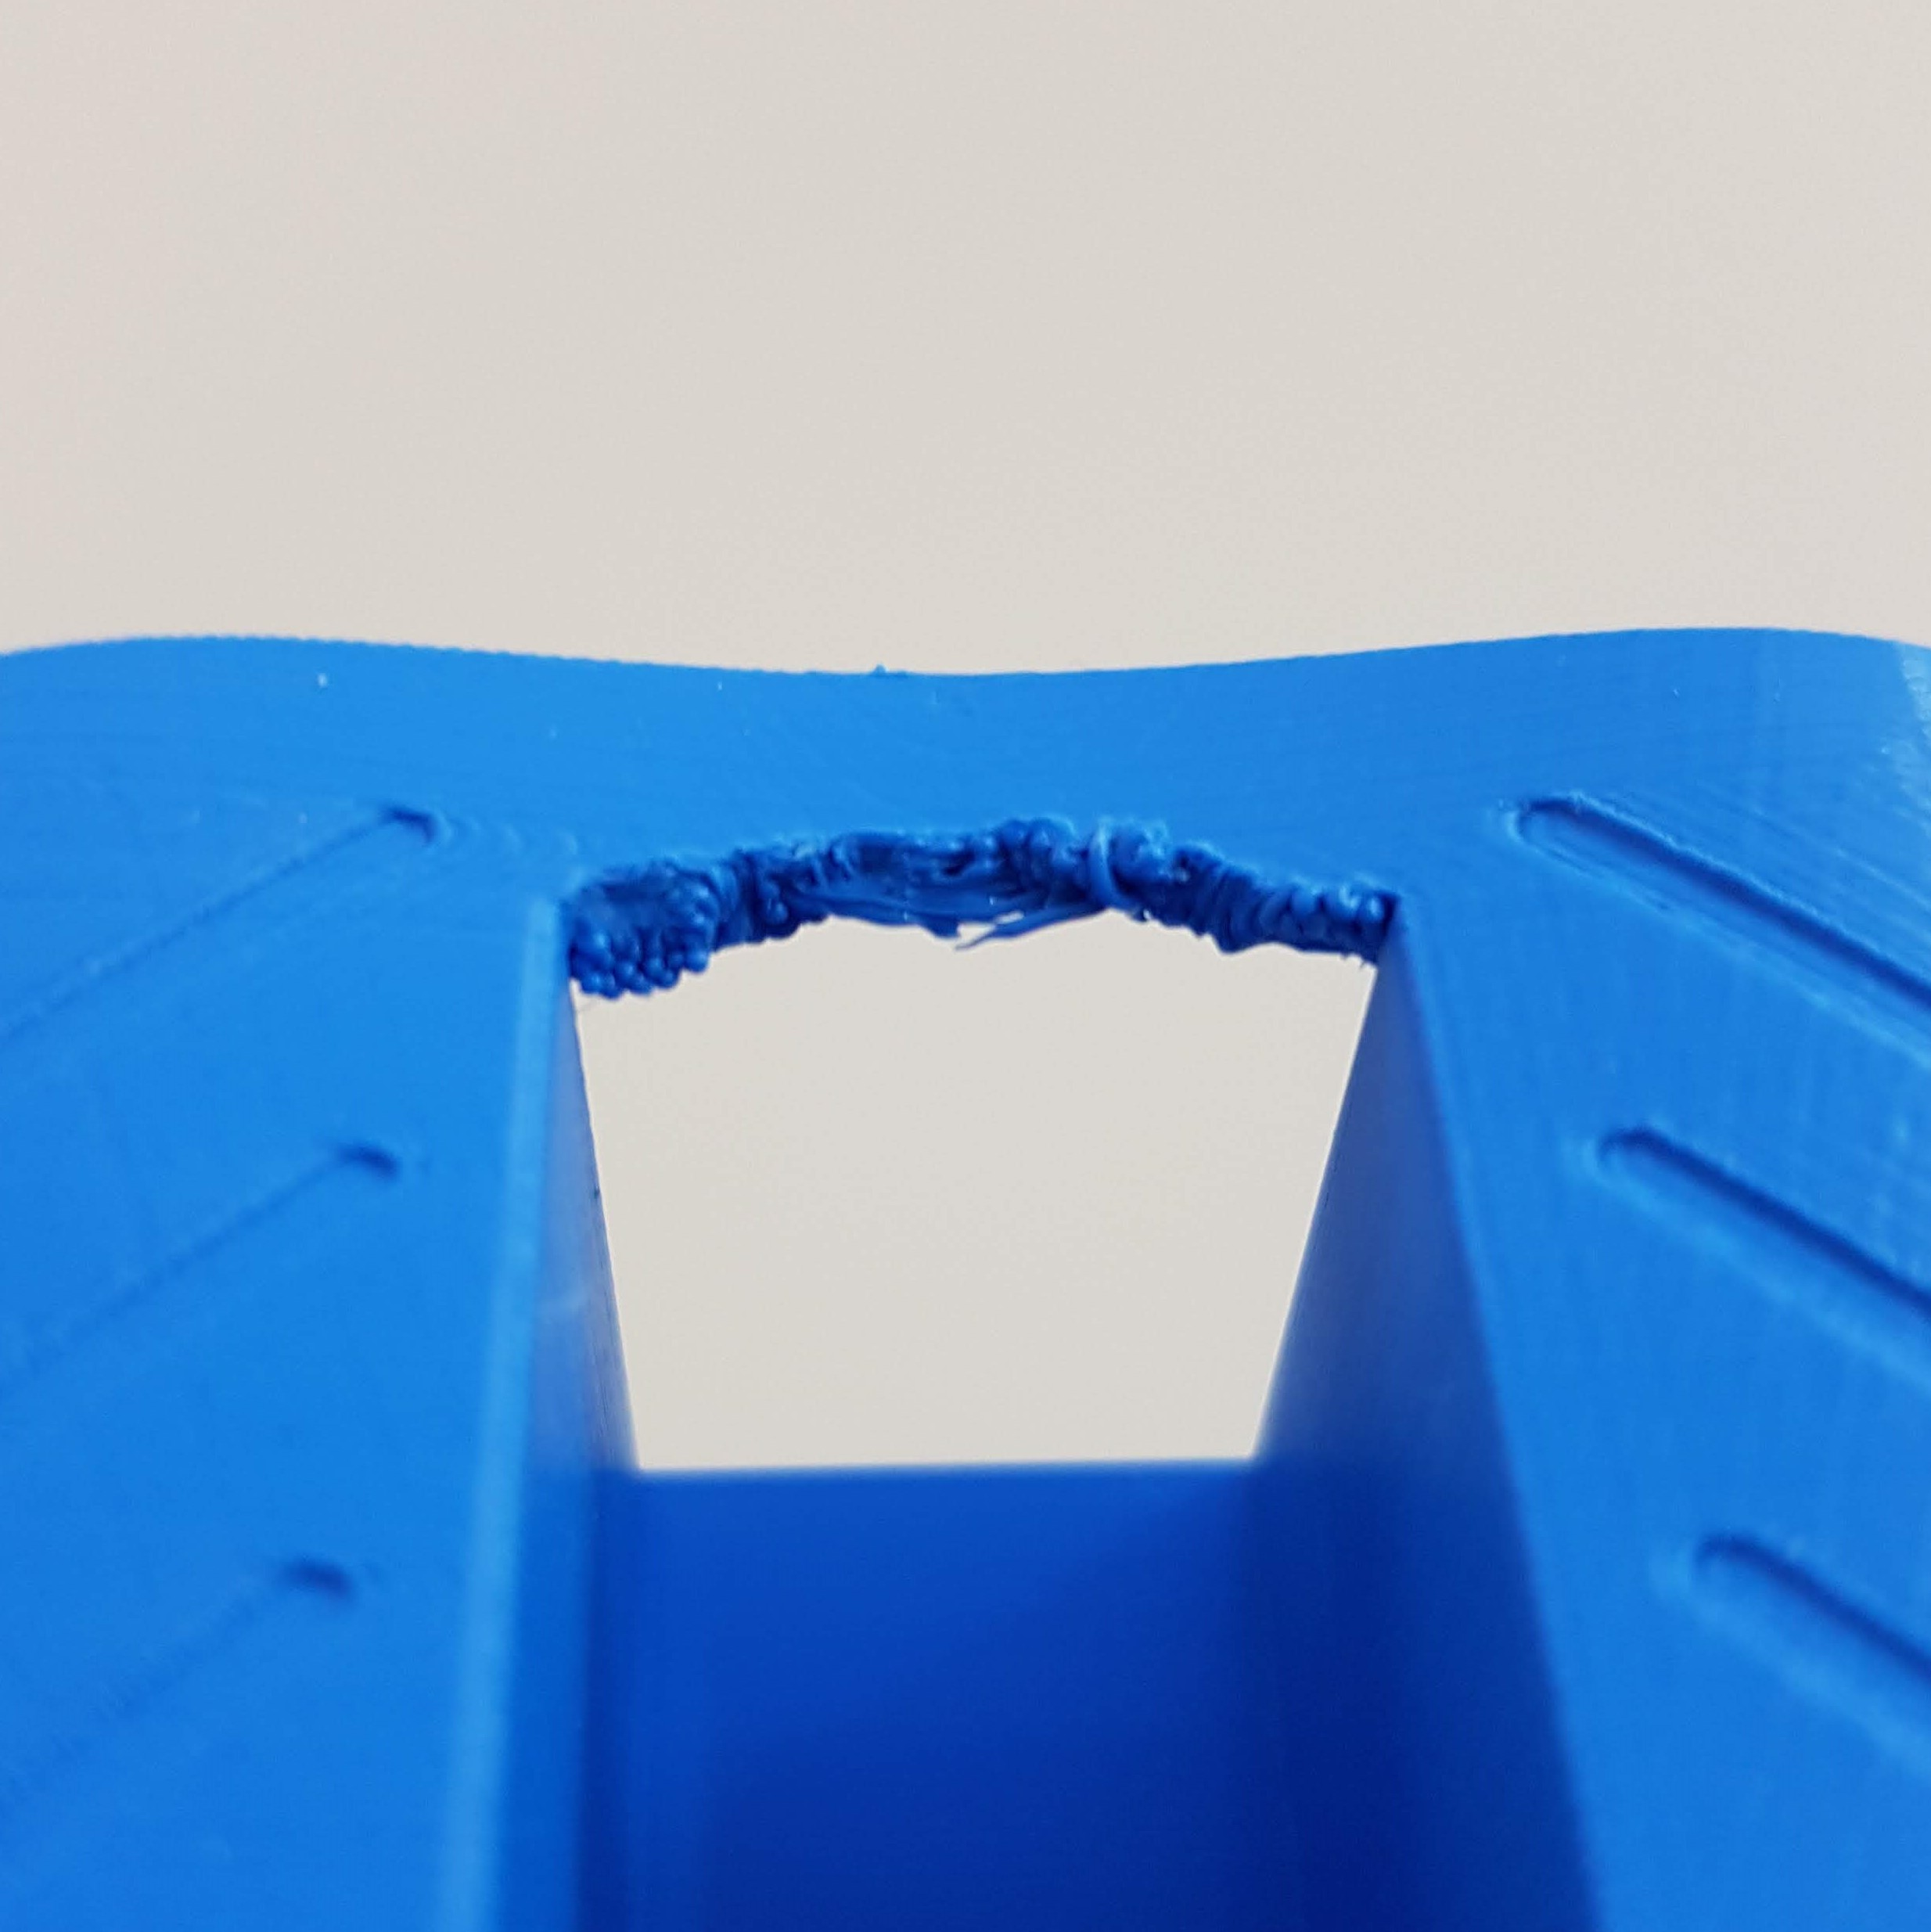
\includegraphics[width=.9\linewidth]{figures/Casing/RoughEdge.jpg}
              \caption{Rough edge caused by lack of support structure, designed in a way that it is only optics issue and can be fix by post processing}
    \end{minipage}
    \begin{minipage}{.45\textwidth}
          \centering
            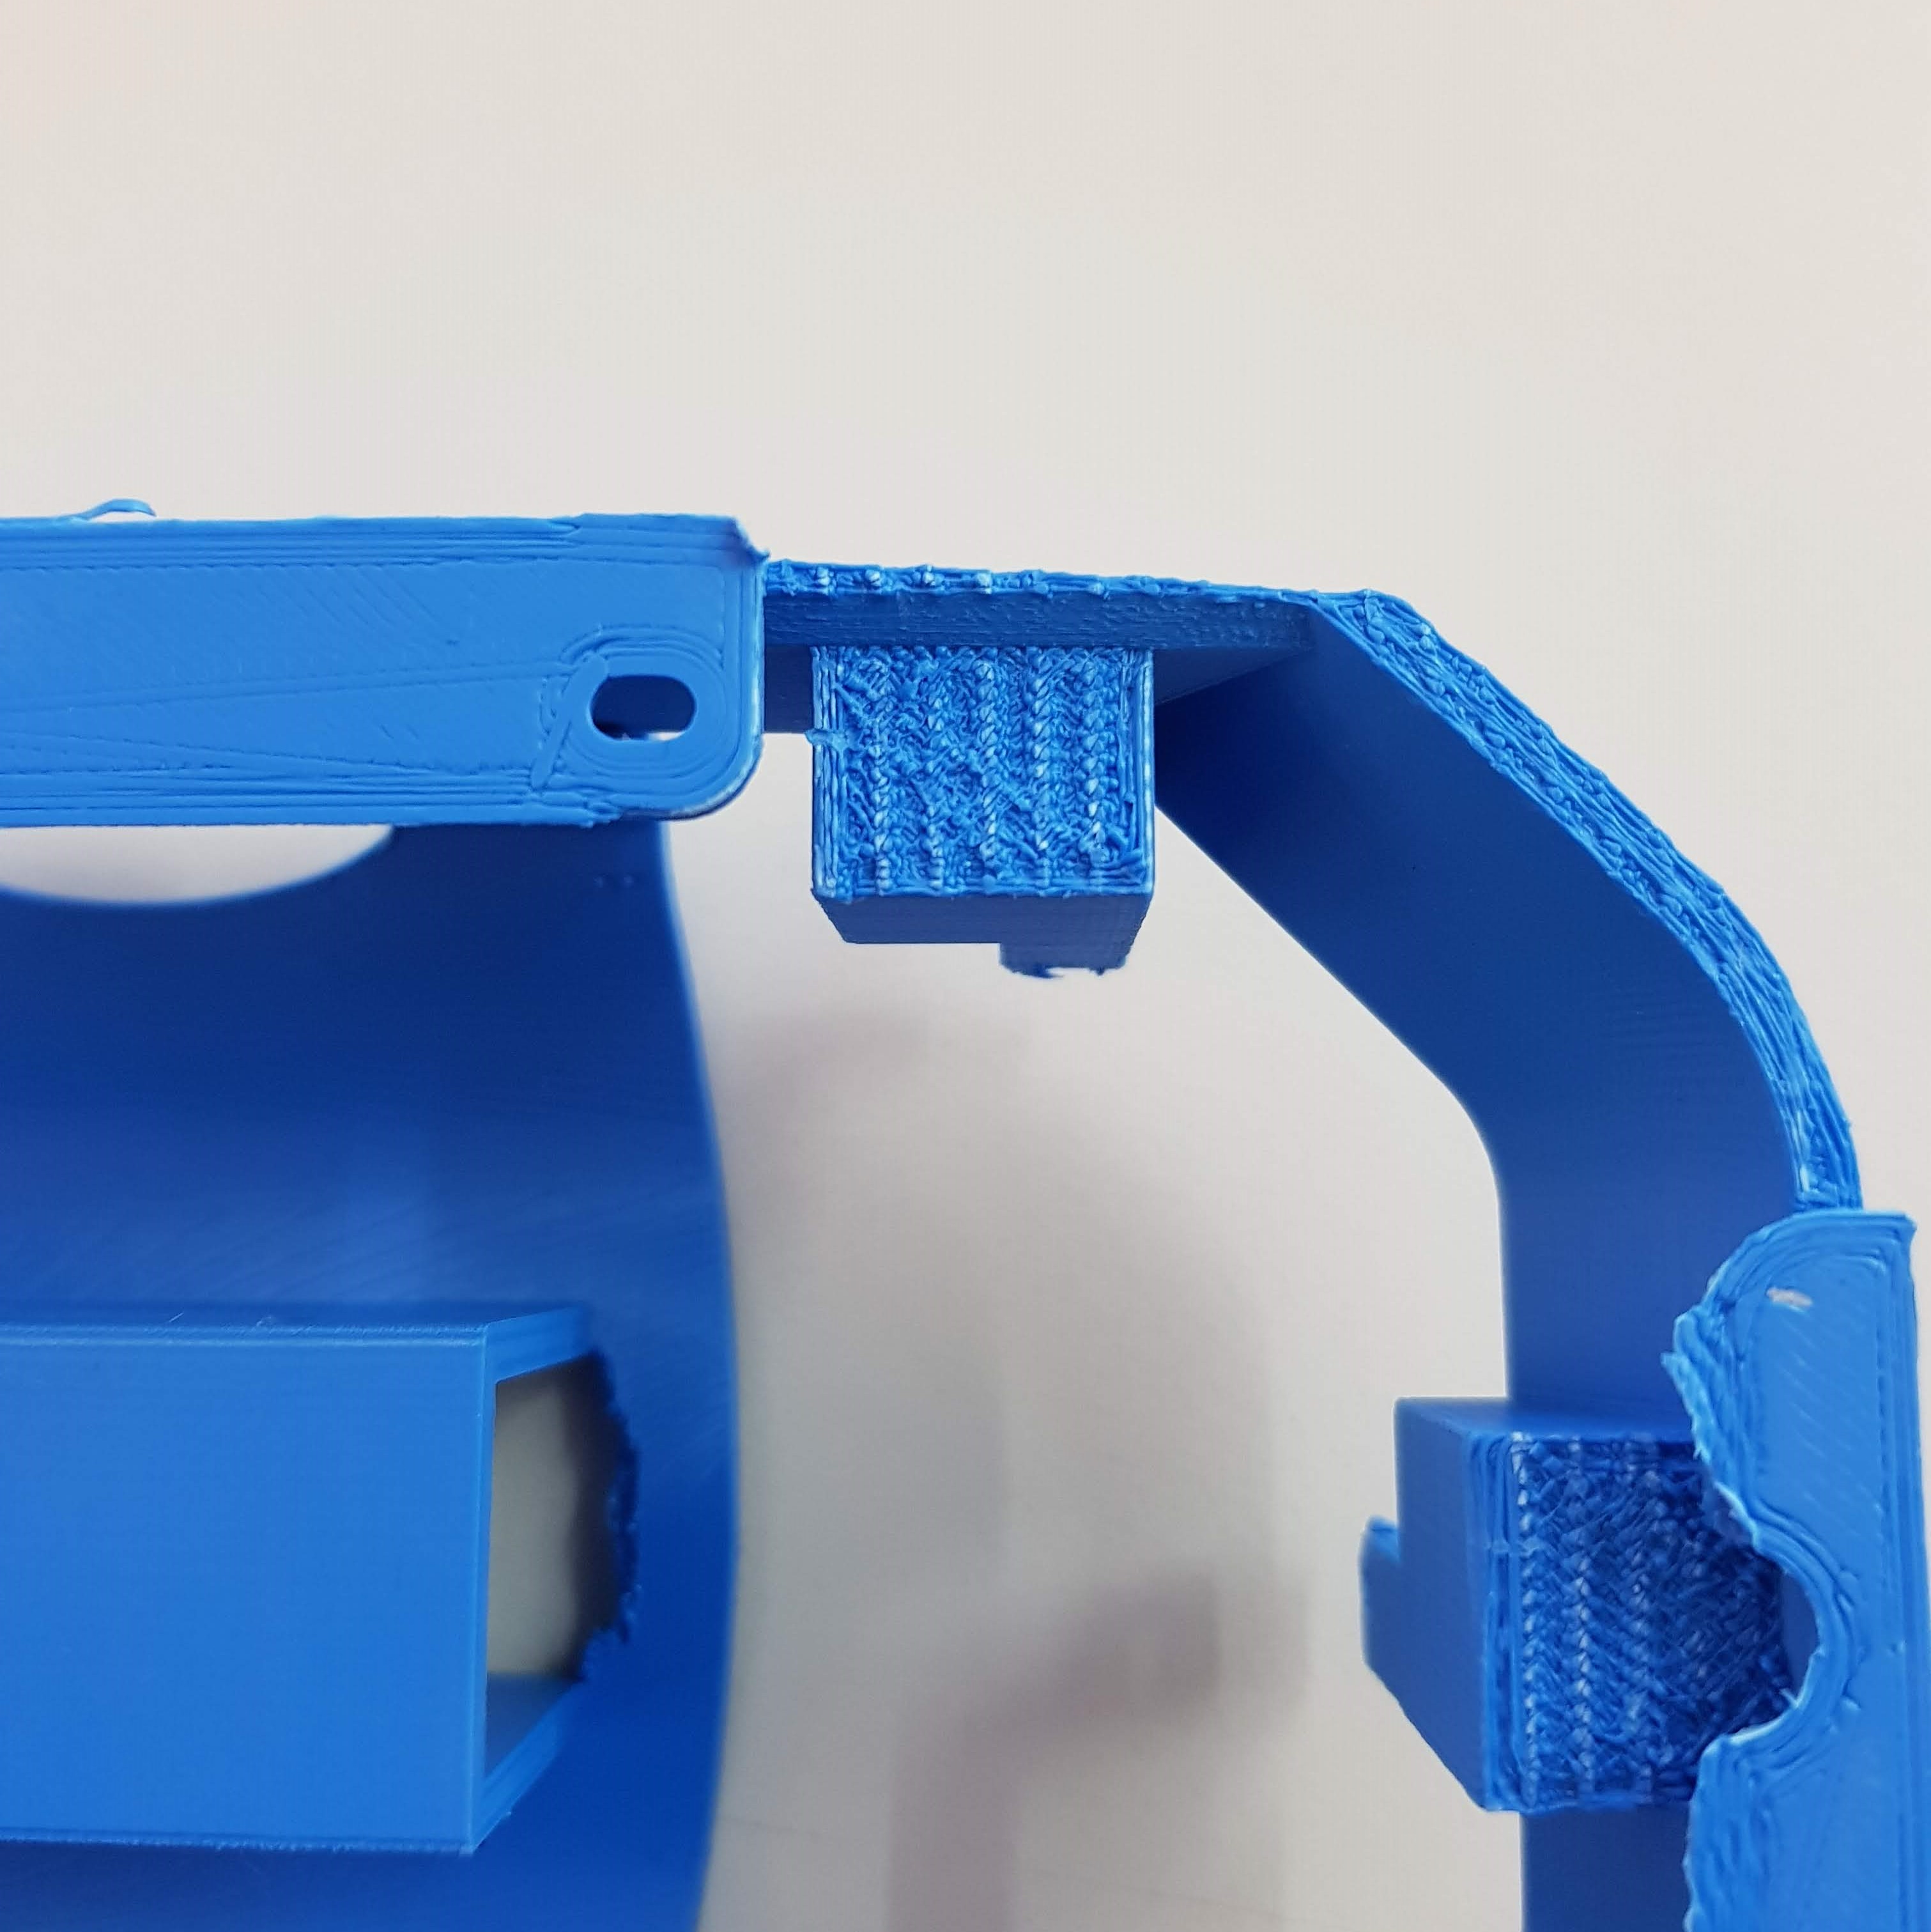
\includegraphics[width=.9\linewidth]{figures/Casing/RoughSurface.jpg}
              \caption{Rough surface after removing support structure, as this is a non-critical surface, it does not cause any functional issues}
                \label{fig:3dprintroughsurface}
    \end{minipage}
\end{figure}

      \item Solution found:\\
      To alleviate such problem, it is firstly important to be mindful of the limitations that come with 3D printing, when designing parts that are supposed to be 3D printed. Avoid support structure as much as possible, one helpful thing to keep in mind is the 45 degree rule of FDM printing. It is said that FDM 3D printers can handle a overhanging structure of 45 degree, larger than that the print will deform. Therefore, by utilising this design rule, many overhanging structures can be avoided. Since support structures leave rough edges, it is important to identify the critical surfaces that require a high precision and accuracy to not have support structures, these surfaces are called critical surfaces. These critical surfaces are identified, such as inside wall of sensor casing, and designed in a way that they do not need support structures. However, it is sometimes difficult to avoid such support structures, it is then best to place support structures on non-critical surfaces, so that the negative consequence is only optical rather than functional, see figure \ref{fig:3dprintroughsurface}.
      
      Second, when printing, a well chosen printing configuration can also help. Sometimes just by rotating the angle, at which the part is printed, can save a lot of support structures, by utilising the 45 degree rule.
      
      Lastly, when support structures are unavoidable, for example when there is a ring like structure, it would then be necessary to post-process the printed part by sanding, polishing etc.
  \end{itemize}
\end{enumerate}
